\documentclass[11pt]{article}
\usepackage[english,serbian]{babel}
\usepackage{graphicx}
\usepackage{epsfig}
\begin{document}
\section{Uvod}
    

    Zvuk je vibracija koja se širi kroz vazduh (ili neku drugu sredinu) u vidu talasa. Čovek može čuje od 16 do 20000 Hz. Ispod ove granice je infrazvuk, a iznad ultrazvuk. Osnovne karakteristike zvuka su visina, boja i jačina.
    \begin {itemize}
        \item[-] Visina zvuka određena je njegovom osnovnom frekvencijom (više tonove stvaraju talasi
        veće frekvencije i obrnuto).
    
        \item[-] Boja zvuka je određena karakterom oscilovanja zvučnih talasa. Obično, zvuk nije prost
        harmonijski talas, već je složen iz viših harmonika. Složenost talasa, broj i spektar viših
        harmonika određuje boju zvuka. Parni harmonici daju zvuku toplinu i mekoću, a neparni
        oštrinu i hladnoću.
    
        \item[-] Jačina zvuka (I) određena je količinom energije koju zvučni talas prenese u jedinici
        vremena kroz jediničnu površinu koja je normalna na pravac prostiranja talasa. Izražava se
        u vatima po kvadratnom metru.
    \end{itemize}
    \centering 
    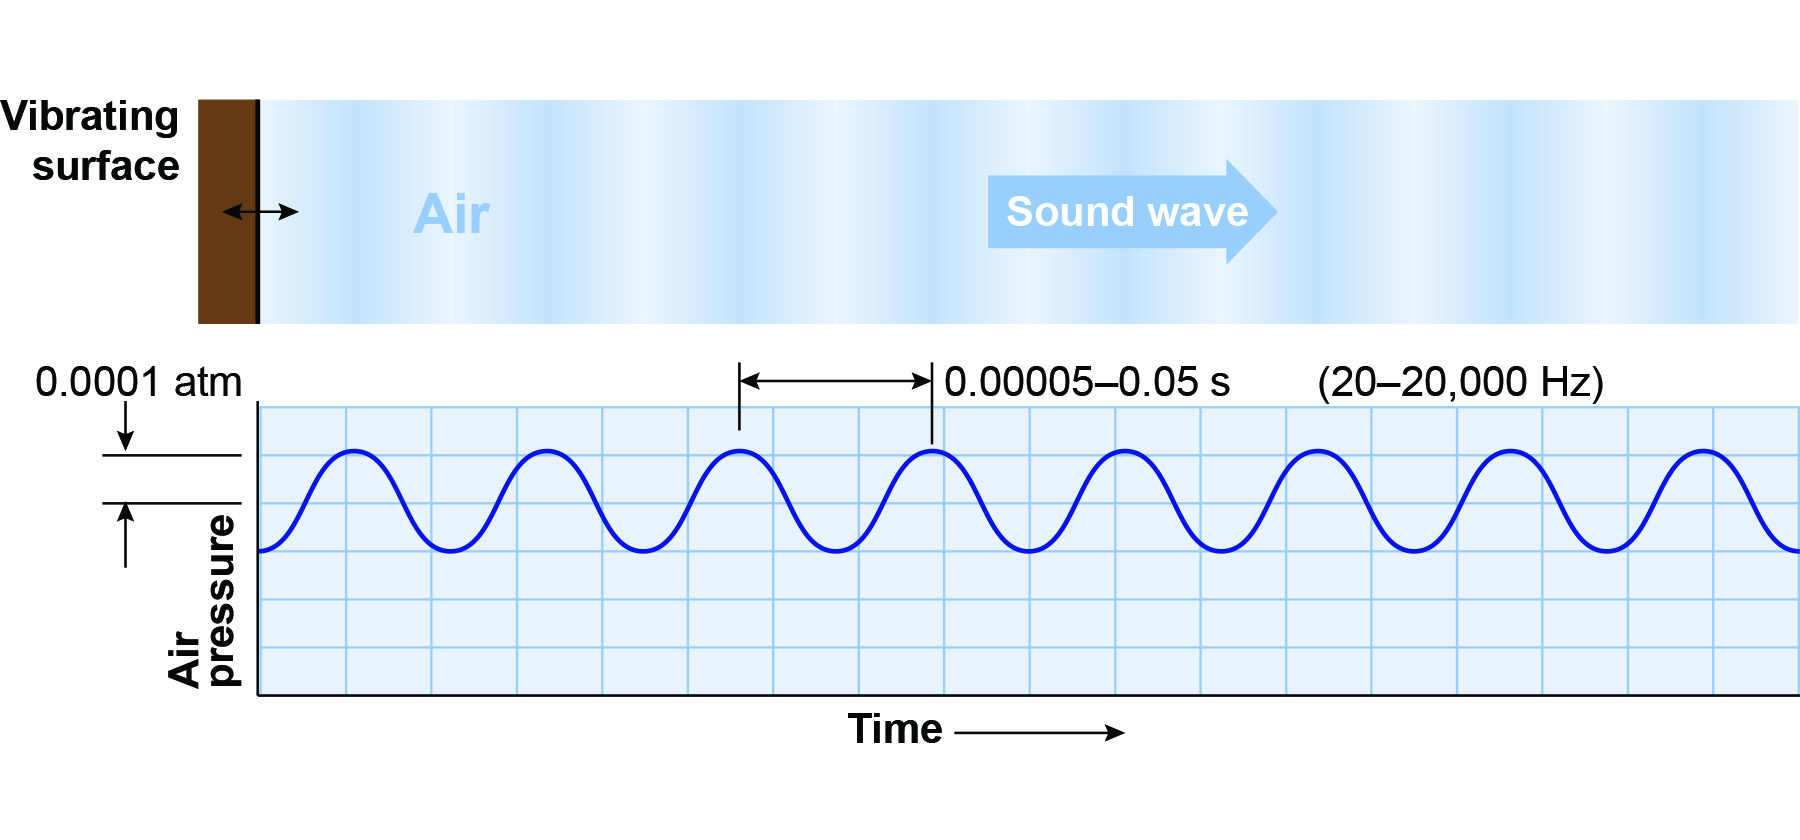
\includegraphics[width=0.8\textwidth]{airpressure}
    \begin{flushleft}
    \section{Kratka istorija digitalizacije}
\end{flushleft}
\end{document}